


\newpage
\section{Cahn Hilliard Equation on a Closed Membrane}%
\label{sec:cahn_hilliard_equation}


Let $c_0$ and $c_1$  indicate the concentration profile of the substances in a a $2$ -phase system such
that $c_0 \left( \mathbf{x},t \right): \Omega  \times \left[ 0, \infty \right] \to \left[ 0,1 \right]$ and
similarly $c_1 \left( \mathbf{x},t \right): \Omega \times \left[ 0, \infty \right] \to \left[ 0,1 \right]$, where
$\mathbf{x} $ is a element of some surface $\Omega $ and $t$ is time.
However, in the $2$ phase problem will we will restrict ourself so that $c_0\left( t,\mathbf{x} \right) + c_1\left( t,
\mathbf{x} \right) = 1$ at any $\mathbf{x} $ at time $t$. A property of the restriction is that we now can express
$c_0$ using $c_1$, with no loss of information. Hence, let us now define $c = c_0$ so $c \left( \mathbf{x},t \right):
\Omega  \times \left[ 0, \infty \right] \to \left[ 0,1 \right]$. It has been shown that $2$ phase system if
thermodynamically unstabl can be evolve
into a phase seperation
described by a evolutional differential equation \cite{cahnhilliard1957} using a model based on chemical energy of the
substances. However, further development has been done \cite{yushutin19} to solve this equation on surfaces. Now assume
model that we want to describe is a phase-seperation on a closed membrane surface $\Gamma $, so that $c \left( \mathbf{x},t \right):
\Gamma \times \left[ 0, T \right] \to \left[ 0,1 \right]$. Then is the surface Cahn Hilliard equation described such that

\begin{equation}
    \label{eq:cahn1}
\rho \frac{\partial c}{\partial  t}  - \nabla_{\Gamma } \left( M \nabla _{\Gamma } \left( f_{0}'  - \varepsilon ^2
        \nabla^2
_{\Gamma } c \right) \right) = 0  \quad \text{on } \Gamma
.\end{equation}

We define here the tangential gradient operator to be $\nabla _{\Gamma } c = \nabla c - \left( \mathbf{n} \nabla c
\right)\mathbf{n} $ applied on the surface $\Gamma $ restricted to $\mathbf{n} \cdot \nabla _{\Gamma } c = 0$.

Lets define $\varepsilon $ to be the size of the layer between the substances $c_{1}$ and $c_{2}$. The density $\rho $ is
simply defined such that $\rho = \frac{m}{S_{\Gamma }}$ is a constant based on the total mass divaded by the total
surface area of $\Gamma $.
Here is the mobility $M$ often derived such that is is dependent on $c$ and is crucial for the result during a possible
coarsering event \cite{yushutin19}.  However, the free energy per unit surface
$f_{0} = f_{0}\left( c \right)$ is derived based on the thermodynamical model and should according to \cite{yushutin19} be nonconvex and
nonlinear.

A important observation is that equation \eqref{eq:cahn1} is a fourth order equation which makes it more challenging to
solve using conventional FEM methods. This clear when writing the equation on the equivalent weak form and second order
equations arise.


\section{$C^0$ Interior Penalty Method}
\label{sec:ch1}

\subsection{Introduction of the Boundary Value Problem}%
\label{sub:introduction_of_the_bvp}


In this section do we want to establish a numerical method to fourth order equations. Instead of embarking on the
special case of surface PDE described in \eqref{eq:cahn1} can we establish a general numerical theory on $\mathbb{R} ^2$, which we later can generalize on closed surface later. Assume that we restrict ourself to a compact surface $\Omega \in \mathbb{R} ^2 $ and let $f \in L^{2}\left( \Omega
\right) $ as defined in \ref{sub:l_2_space}.
Let say we want to solve the equation on the form.

\begin{equation}
\label{eq:ch1_bvp}
\begin{split}
    \Delta ^2 u - \beta \Delta u + \gamma u &= f \quad \beta , \gamma \ge 0 \\
    \frac{\partial u}{\partial  n}  &= 0 \quad \text{on }\Omega  \\
    \frac{\partial \Delta u}{\partial  n}  &= q \quad \text{on } \partial \Omega  \\
\end{split}
.\end{equation}

For convenience are the boundary condition $q$ chosen to be defined via a  $\phi \in H^{4}\left( \Omega  \right)$
such that $q = \frac{\partial \Delta \phi }{\partial  n} $ so $\frac{\partial \phi }{\partial  n}  = 0$.
$\partial \Omega $.


\subsection{Weak Formulation}%
\label{sub:weak_formulation}

We want to rewrite \eqref{eq:ch1_bvp} on weak formulation. Now define the Hilbert space \[
V = \left\{ v \in H^2\left( \Omega  \right): \frac{\partial v}{\partial  n}  = 0 \quad \text{on } \partial \Omega
\right\}.
\]
It can be shown \cite{gu2012c0} that a convinient form is to write it as
\begin{equation}
\label{eq:weakform}
    \begin{split}
a\left( u,v \right) &=  \left( f,v \right)_{L^2\left( \Omega  \right)}  - \left( q,v \right)_{L^2\left( \partial \Omega  \right)}  \\
& = \int_{\Omega }^{} D^2 w : D^2 v dx +  \int_{\Omega }^{} \nabla w \nabla v dx + \int_{\Omega }^{} \gamma w \cdot v dx
.\\
    \end{split}
.\end{equation}
For all $\forall v \in  V$, where \[
D^2 w : D^2 v = \sum_{i,j=1}^{2}  \frac{\partial ^2 w}{\partial x_{i} \partial x_{j} } \cdot  \frac{\partial ^2 v
}{\partial x_{i} \partial x_{j} }.
\]

Abusing notation can we see this is clearly arise since \[
    \begin{split}
\int_{\Omega }^{} \Delta ^2 w \cdot  v   dx & = - \int_{\Omega }^{} \nabla \left( \Delta w \right) \nabla v dx \\
&= \int_{\Omega }^{} \Delta w \Delta v dx  -\int_{\partial \Omega }^{} \nabla v \frac{\partial \Delta w}{\partial n } ds   \\
&= \left( \Delta w, \Delta v \right)_{L^2\left( \Omega  \right)} - \left( q,v \right) _{L^2\left( \partial \Omega  \right)} \\
    \end{split}
\]
\todo[inline]{ why is minus sign in front of $\left( q,v \right) _{L^2\left( \partial \Omega  \right)}$ and is it
correct to use $q$ in this setting? I also wonder how  $ \left( \Delta w, \Delta v \right)$ appears to be $\left( D ^2
w, D^2 v \right)$ at some point.}

In fact, according to \cite{gu2012c0} can it be shown that the problem has a unique solution if and only if $\gamma >
0$. However, in the case where $\gamma  = 0$ can we provoke a unique solution by introducing the condition \[
\int_{\Omega }^{} f dx = \int_{\partial \Omega }^{}  q ds
\]

Taking this into account can we expand the solution space such that \[
V^* = \begin{cases}
    V, \quad & \text{if } \gamma >0 \\
    \left\{ v \in V: v\left( p^* \right) = 0 \right\}, \quad & \text{if } \gamma  =0
\end{cases}
\]

Where $p^{*}$  is a corner in $\Omega $. In fact, now all solutions of \eqref{eq:weakform} exists in $V^{*}$.


\subsection{Construction of $C^{0}$ Interior Penalty Method}%
\label{sub:construction_interior_penalty_method}

We want to construct a $C^{0}$ interior penalty method based on $C^{0}$ Lagrange elements.
Assume $\mathcal{T}_{h} $ be a tringaluation of $\Omega $ and $V_{h}$ be the a $\mathcal{P}_{2} $ Lagrange finite
element space associated with $\mathcal{T}_{h} $ \[
V_{h} = \left\{ v \in C\left( \overline{\Omega } \right) : v_{T} = v |_{T} \in \mathcal{P}_{2}\left( T \right) \quad
\forall T \in  \mathcal{T} _{h}  \right\}
\]
So that we can earn a similar space for the approximated solution space ,
\[
V_{h}^{*} = \begin{cases}
    V_{h}, \quad & \text{for } \gamma >0\\
    \left\{ v \in V_{h}: v\left( p^{*} \right) = 0 \right\} \quad & \text{for } \gamma = 0.
\end{cases}
\]
Here is $p^{*}$ again a corner in $\Omega $. Let us now generelize the Hilbert space as well to the approximated
solution space by defining \[
H^{k}\left( \Omega , \mathcal{T} _{h}  \right) = \left\{ H^{1}\left( \Omega  \right): v_{T} \in H^{k}\left( T
\right)\quad \forall T \in \mathcal{T} _{h} \right\}.
\]
\begin{figure}[!h]
\centering
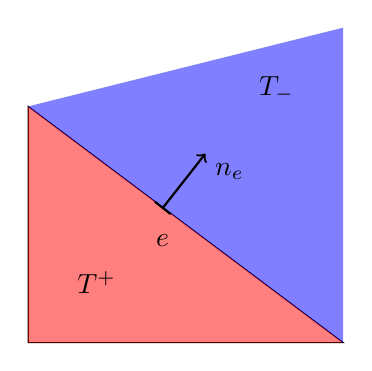
\begin{tikzpicture}[scale=1]
\coordinate (A) at (0,0);
\coordinate (C) at (0,3);
\coordinate (B) at (4,0);
\coordinate (D) at (4,4);
\coordinate (Tm) at (3.5,3.5);
\coordinate (Tp) at (0.5, 0.5);
\coordinate (e) at (1.5, 1.5);
\coordinate (start) at (1.7, 1.7);
\coordinate (end) at (2.25, 2.4);

\draw (A) -- (B) -- (C) -- cycle;
\fill[red, opacity=0.5] (A) -- (B) -- (C);
\fill[blue, opacity=0.5] (B) -- (C) -- (D);
\node[below left] at (Tm) {$T_{-} $ };
\node[above right] at (Tp) {$T^{+}$ };
\node[below right] at (e) {$e$ };

\draw [|->, thick] (start) -- (end);
% \node[above right] at (A) {A };
% \node[below right] at (B) {B};
% \node[above right] at (C) {C };
% \node[below right] at (D) {D};
\node[below right] at (end) {$n_e$};
\end{tikzpicture}
\caption{Edge $e$ shared by the triangles $T_{-}$ and $T_{+}$ and the normal unit vector $n_{e}$.  }
    \label{fig:normal}
\end{figure}

Now assume that that $e \in \mathcal{E}_{h}^{i} $ is shared between two triangles $T_{-}, T_{+} \in  \mathcal{T} _{h}$ .
Then we can assume that the unit normal from $T_{-}$ to $T_{+}$ is described as $n_{e}$ as illustraded in figure
\ref{fig:normal}. Finally, we now want to define jumps internally, \[
\begin{split}
    \jump{ \frac{\partial v_{h}}{\partial n_{e}} } &= \frac{\partial v_{T_{+}}}{\partial n_{e}  } | _{e} -
    \frac{\partial v_{T_{-}}}{\partial n_{e}  } |_{e}, \quad \forall v \in H^{2}\left( \Omega , \mathcal{T} _{h} \right)  \\
    \jump{ \frac{\partial ^2 v_{h}}{\partial n_{e} ^2 } } &= \frac{\partial ^2 v_{T_{+}}}{\partial  n_{e}^2} |_{e}  -
    \frac{\partial ^2 v_{T_{-}}}{\partial n_{e}^2   } |_{e} \quad \forall v \in H^3\left( \Omega , \mathcal{T} _{h}
    \right).  \\
\end{split}
\]

And similarly for means internally,
\[
    \begin{split}
\mean{ \frac{\partial v_{T_{-}}}{\partial n_{e} } } &= \frac{1}{2} \left( \frac{\partial v_{T_{+}}}{\partial n_{e} }
|_{e} +  \frac{\partial v_{T_{-}}}{\partial n_{e} } |_{e}  \right) \quad  \forall v \in H^2\left( \Omega , \mathcal{T}
_{h} \right) \\
    \mean{ \frac{\partial ^2 v_{h}}{\partial n_{e}^2 } } &= \frac{1}{2} \left( \frac{\partial ^2 v_{T_{+}}}{\partial
    n_{e}^2  } + \frac{\partial ^2 v_{T_{-}}}{\partial n_{e}^2  }    \right) \quad \forall v \in  H^3\left( \Omega .
\mathcal{T}_{h}  \right), \\
    \end{split}
\]

Let the edges along the boundary be defined as $e \in  \mathcal{E} _{h}^{b}$ along a some boundary triangle $\mathcal{T}
_{h}$. We can then define the jump and mean as \[
\begin{split}
    \jump{ \frac{\partial v_{h} }{\partial n_{e} } } & = -\frac{\partial v_{T}}{\partial  n_{e}} |_{e} \quad \forall v \in
    H^2\left( \Omega , \mathcal{T}_{h}  \right) \\
    \mean{ \frac{\partial ^2 v_{h}}{\partial n_{e}^2 } } & = \frac{\partial v_{T}}{\partial  n_{e}} |_{e} \quad \forall v \in
    H^3\left( \Omega  , \mathcal{T}_{h}  \right)
\end{split}
\]


